%!TEX TS-program = pdflatex
%!TEX encoding = UTF-8 Unicode

\documentclass[11pt]{article}

\usepackage[utf8]{inputenc}
\usepackage{geometry}
\geometry{a4paper}
\usepackage{graphicx}
\usepackage{booktabs}
\usepackage{array}
\usepackage{verbatim}
\usepackage{subfig}
\usepackage{hyperref}

\usepackage{url}

\usepackage{fancyhdr} 
\pagestyle{fancy}
\renewcommand{\headrulewidth}{0pt} 
\lhead{}\chead{}\rhead{}
\lfoot{}\cfoot{\thepage}\rfoot{}

\usepackage{sectsty}
\allsectionsfont{\sffamily\mdseries\upshape}

\usepackage[nottoc,notlof,notlot]{tocbibind} 
\usepackage[titles,subfigure]{tocloft} 
\renewcommand{\cftsecfont}{\rmfamily\mdseries\upshape}
\renewcommand{\cftsecpagefont}{\rmfamily\mdseries\upshape}

\usepackage[spanish]{babel}
\usepackage{listings}

%%%El documento comienza aqui

\title{\textbf{Proyecto MINESWEEPER}}
\author{\textbf{Jimmy Banchón - Rene Balda}}
\date{\textbf{\today}}
\begin{document}

\bibliographystyle{plain}

\maketitle
\section{\textbf{Introducción}} 
\paragraph{} \noindent
El proyecto {\textbf{MINESWEEPER}}, se basa en un videojuego para un solo jugador con varios niveles de dificultad.
El objetivo de este juego es despejar un campo minado sin detonar una sola mina teniendo como pauta números en los
bloques, los cuales nos indican cuantas minas hay alrededor de éste. También tenemos disponibles  los llamados  {\textbf{FLAG}}
para cubrir las minas aunque para esta ocasión decidimos reemplazarlos con escudos  simplemente por originalidad.
\section{\textbf{Alcance del Proyecto}}

Nuestro proyecto cumplió con las siguientes características:
\begin{enumerate}
\item 
Todas las funcionalidades respectivas en la lógica del juego, tales como generación dinámica de los bloques,
función recursiva de exploración, generación de las minas en el campo de juego sin contar el bloque presionado, de identificación de ganador,
reseteo del juego entre otros.

\item
Implementación de un menú con todas las opciones principales tales como: nuevo juego, puntajes altos, selección de niveles, ventanas de diálogo
de juego perdido, juego ganado.

\item
 Manejo de hilos en nuestra clase {\textbf{clock}} el cual controla el tiempo.

\item
{\textbf{Drag and drop}}.

\item
Implementación del modelo vista controlador.

\item
Implementación de almacenamiento de {\textbf{Scores}} en base de datos {\textbf{SQLite 3}} mediante las clases {\textbf{SQLhelper}} que nos brinda el {\textbf{framework}} 			de android.

\item
Uso de {\textbf{BaseAdapter}} para la colocación de las listas en los  {\textbf{ListView}}, en los cuales se presenta nuestro  {\textbf{score}}.
\end{enumerate}
\paragraph{} \noindent De acuerdo a las características antes listadas se cree que se logro casi por completo todos los requetimientos designados para el desarrollo de este juego, a excepción de la implementación del {\textbf{zoom}} en el {\textbf{drag and drop}}.

\section{Diagramación}
\subsection{\textbf{Diagrama de Casos de Uso}}

				\begin{center}
				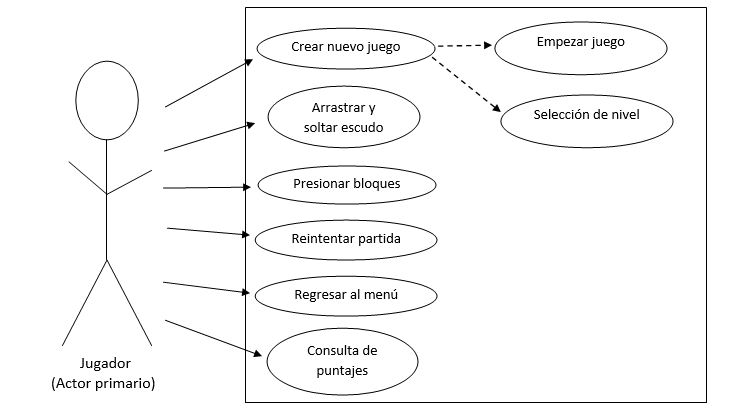
\includegraphics[width=0.8\textwidth]{images/casosDeUso}
				\end{center}

\subsection{\textbf{Diagrama de Clases}}

				\begin{center}
				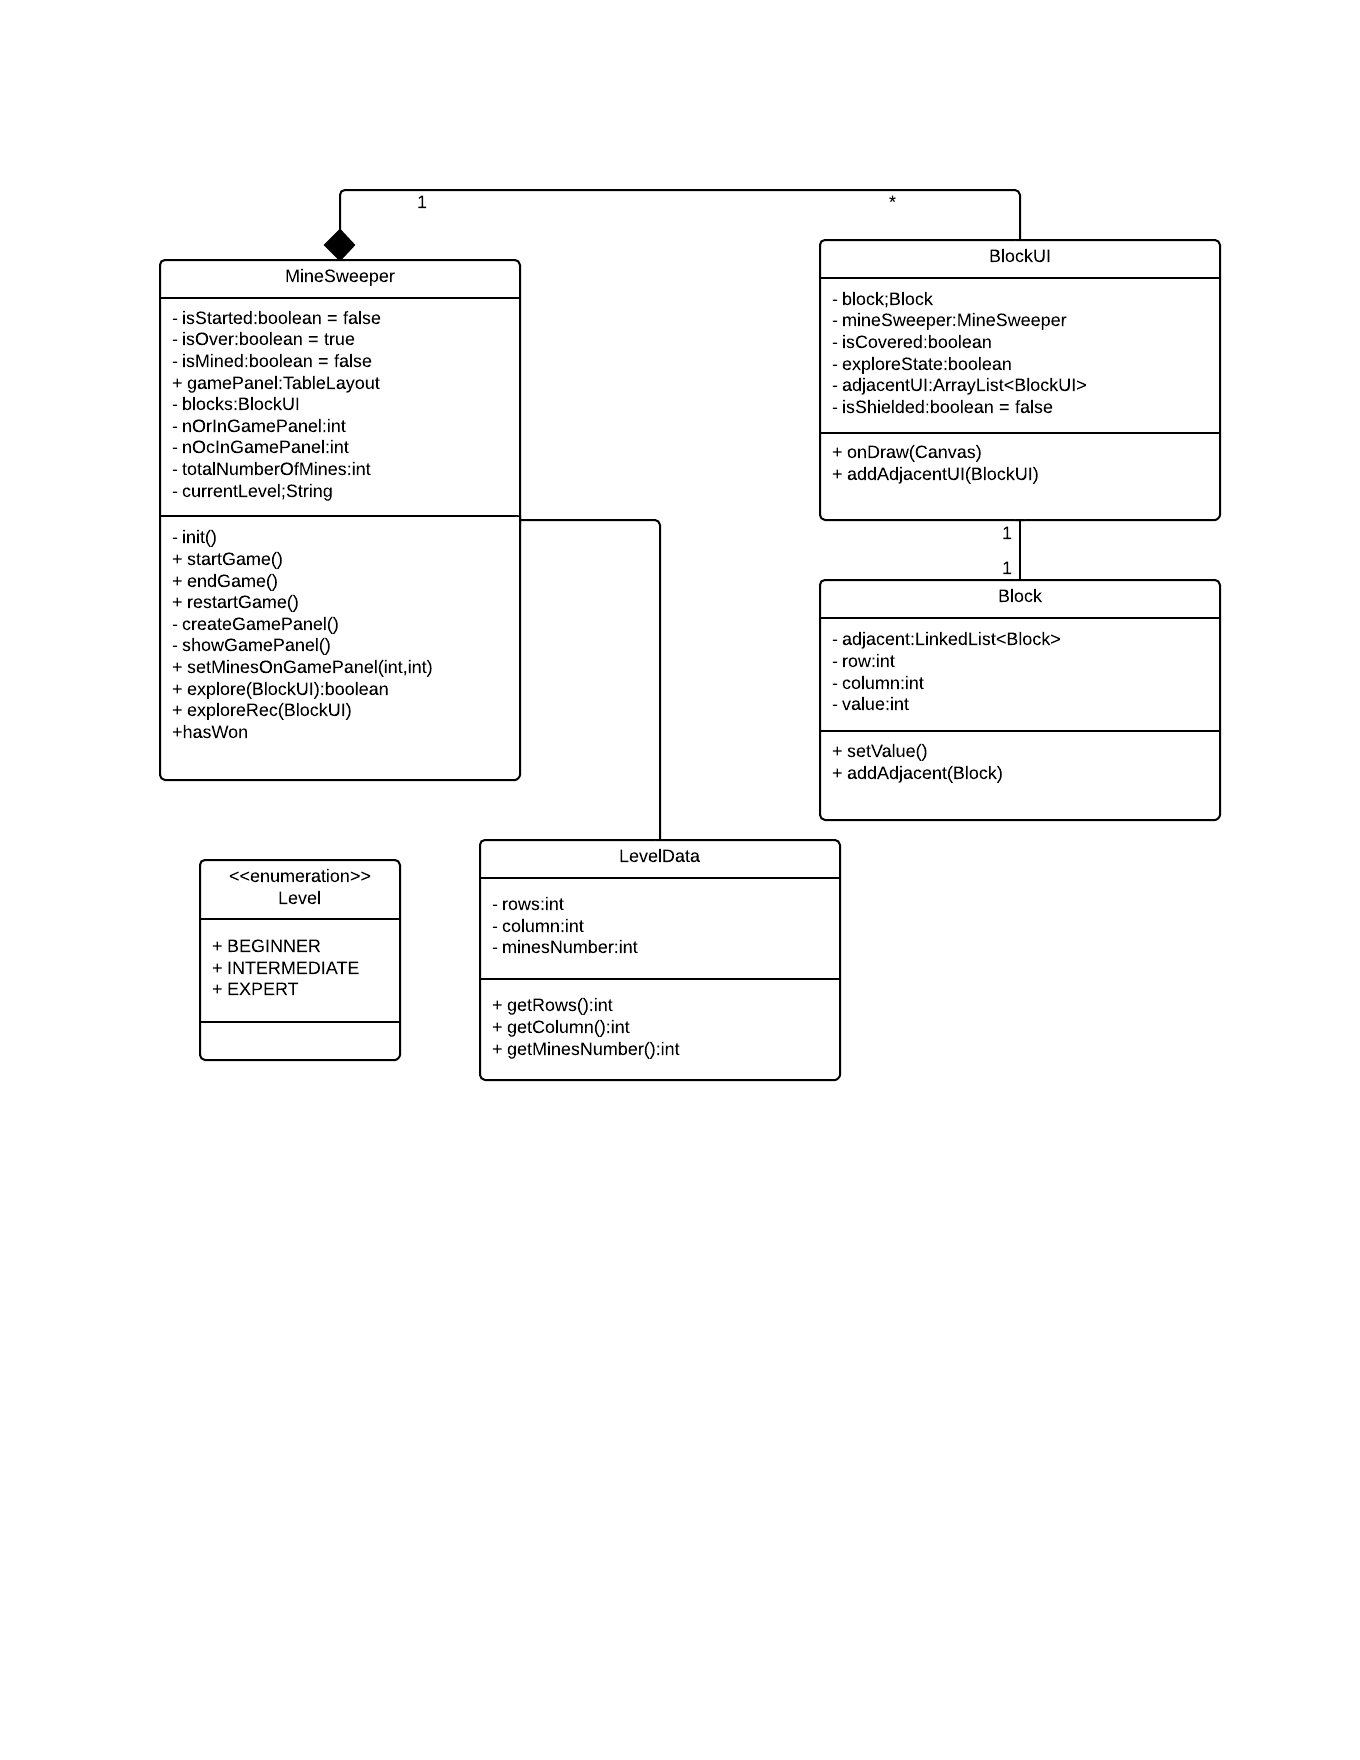
\includegraphics[width=0.71\textwidth]{images/diagramaClase}
				\end{center}

\section{Manual de Usuario}

\begin{figure}[h!]
\begin{minipage}{0.5 \textwidth}
Al ejecutar nuestra aplicación primero obtenemos un menú con diferentes opciones a poder elegir.
\end{minipage}
\hfill \begin{minipage}{6.5cm}
\begin{center}
 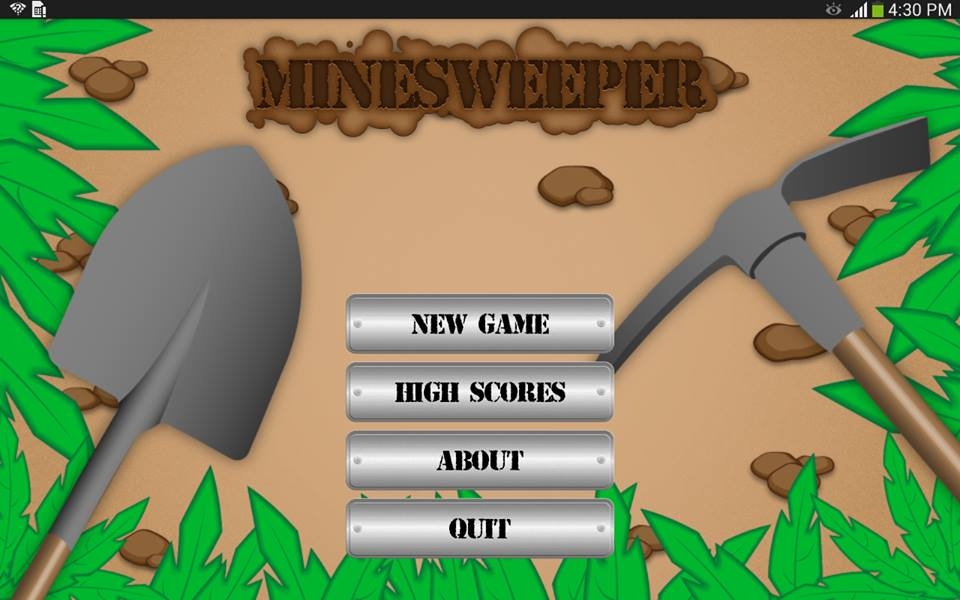
\includegraphics[width=1\textwidth]{images/screenshot1}
\end{center}
\end{minipage}
\end{figure}

\begin{figure}[h!]
\begin{minipage}{0.5 \textwidth}
En caso de escoger nuevo juego nos aparecerá otro menú con el listado de los diversos niveles disponibles más un boton de retorno en caso de equivocarte en tu elección.
\end{minipage}
\hfill \begin{minipage}{6.5cm}
\begin{center}
 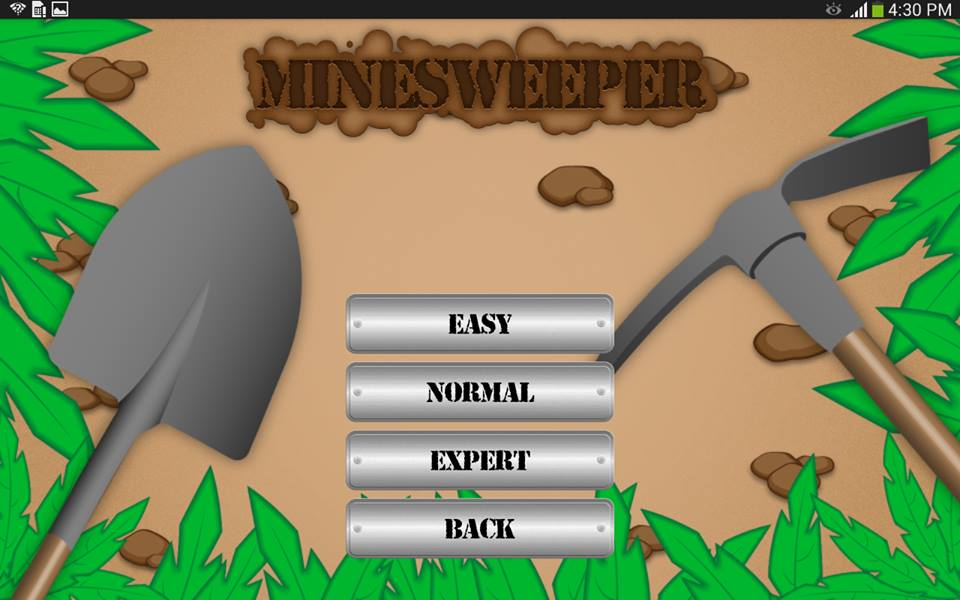
\includegraphics[width=1\textwidth]{images/screenshot2}
\end{center}
\end{minipage}
\end{figure}

\begin{figure}[h!]
\begin{minipage}{0.5 \textwidth}
Después de haber escogido el nivel que deseamos nos aparecerá esta pantalla en donde podemos observar que tenemos en la parte superior el tiempo, una carita, los escudo y el marcador de minas respectivamente. La carita nos sirve al igual que el buscaminas clásico como nuestro boton de inicio el cual nos generara el campo minado y empezara contar el tiempo.
\end{minipage}
\hfill \begin{minipage}{6.5cm}
\begin{center}
 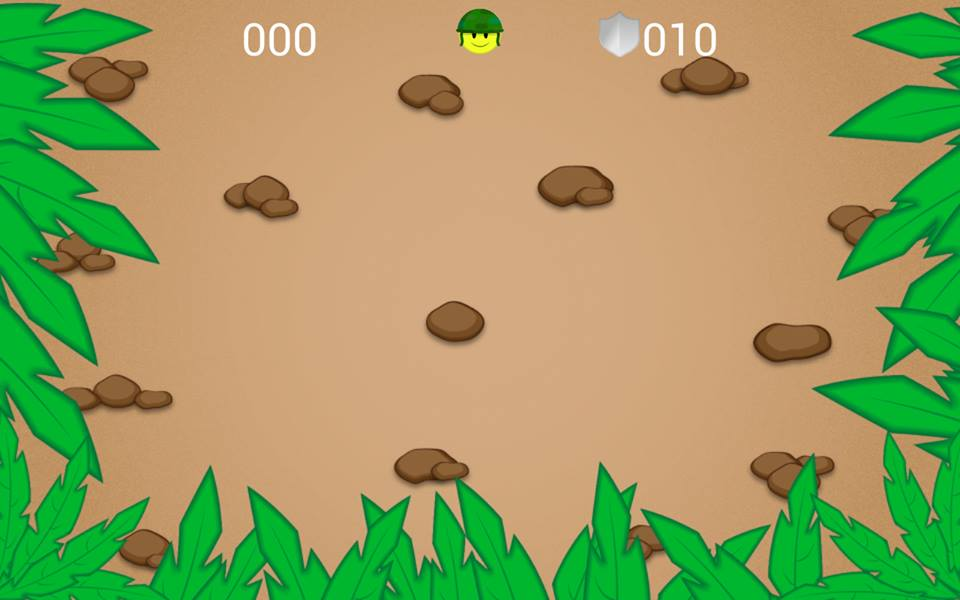
\includegraphics[width=1\textwidth]{images/screenshot3}
\end{center}
\end{minipage}
\end{figure}

\begin{figure}[h!]
\begin{minipage}{0.5 \textwidth}
Una vez tengamos el tiempo contando podremos empezar a jugar presionando cualquiera de los bloques teniendo cuidado que no sea una mina.
\end{minipage}
\hfill \begin{minipage}{6.5cm}
\begin{center}
 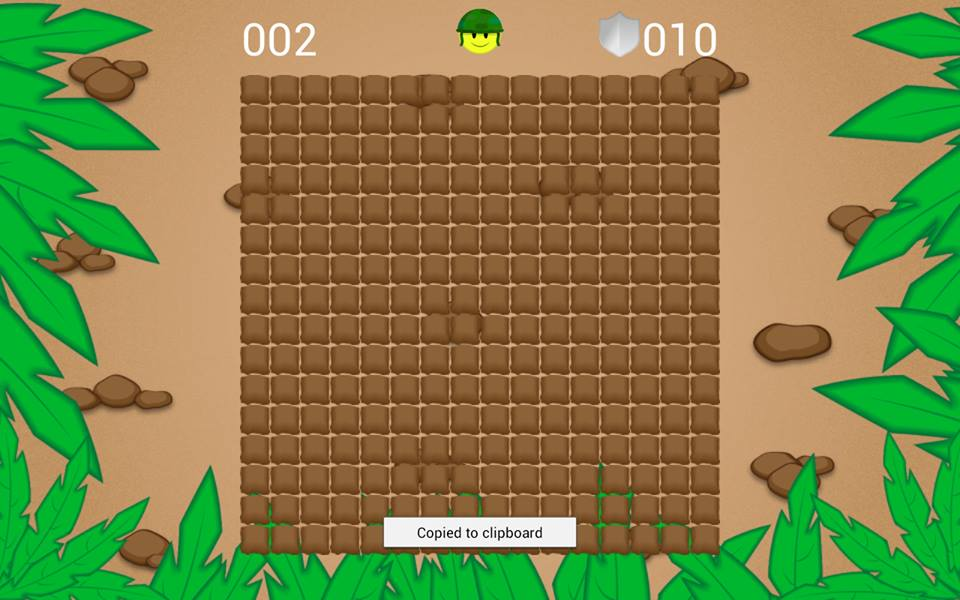
\includegraphics[width=1\textwidth]{images/screenshot4}
\end{center}
\end{minipage}
\end{figure}

\begin{figure}[h!]
\begin{minipage}{0.5 \textwidth}
Después de presionar un botón uno de los casos posibles sería que este nos expanda el campo minado descubriendo mucho de los bloques hasta que se tope con los números los cuáles nos indican que cerca de este se encuentra una mina.
\end{minipage}
\hfill \begin{minipage}{6.5cm}
\begin{center}
 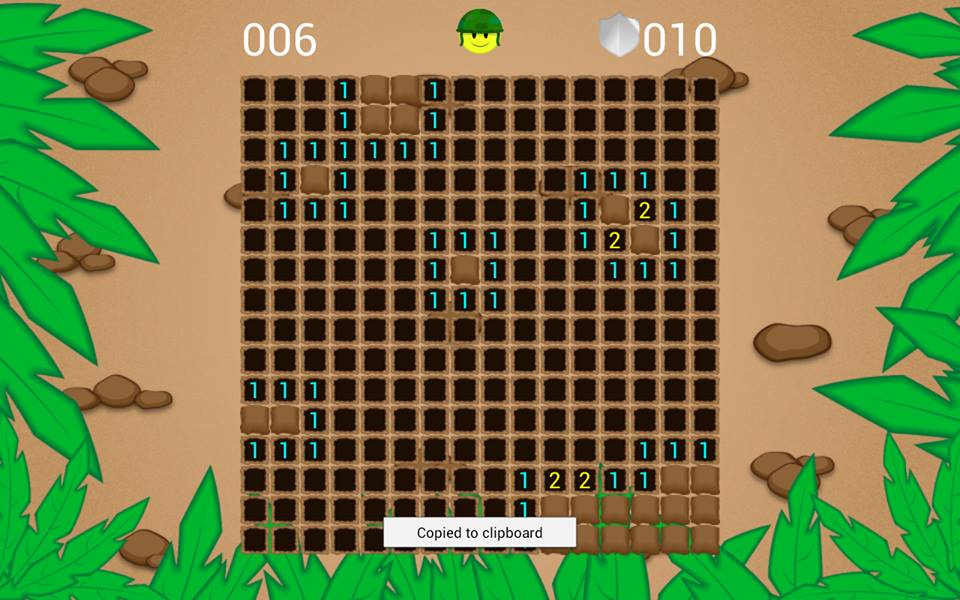
\includegraphics[width=1\textwidth]{images/screenshot5}
\end{center}
\end{minipage}
\end{figure}

\begin{figure}[h!]
\begin{minipage}{0.5 \textwidth}
En el caso de que creamos saber la posición exacta de una de las minas tenemos disponibles los escudos que se encuentran en la parte superior, los cuales los podemos arrastrar y soltar en cualquiera de los bloques que no hayan sido presionados.
\end{minipage}
\hfill \begin{minipage}{6.5cm}
\begin{center}
 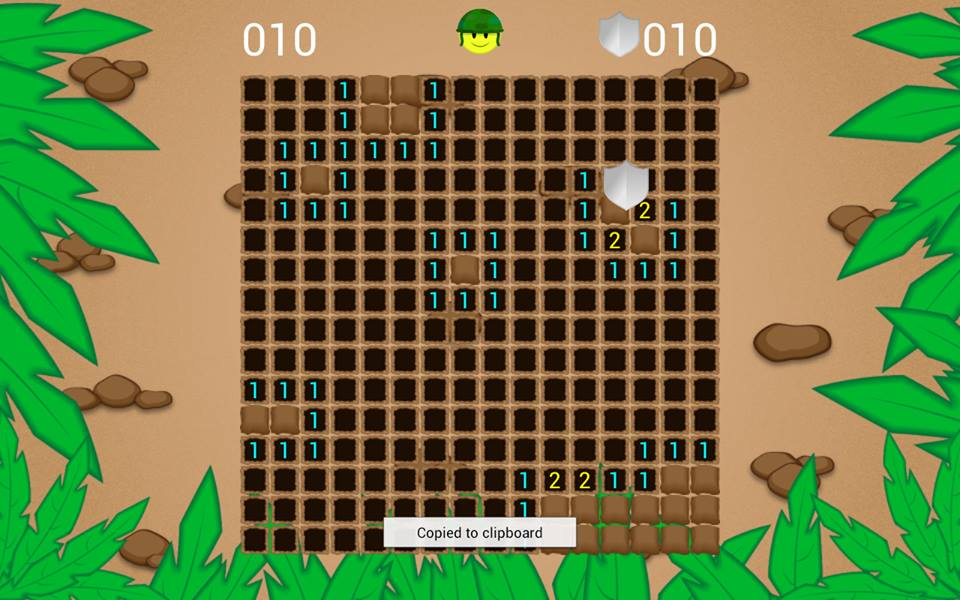
\includegraphics[width=1\textwidth]{images/screenshot6}
\end{center}
\end{minipage}
\end{figure}

\begin{figure}[h!]
\begin{minipage}{0.5 \textwidth}
Al soltar el escudo este se ajustará al bloque haciendo que este ya no pueda ser presionado a menos que muevas el escudo de ahí. Los escudos pueden moverse entre los diferentes bloques no presionados.
\end{minipage}
\hfill \begin{minipage}{6.5cm}
\begin{center}
 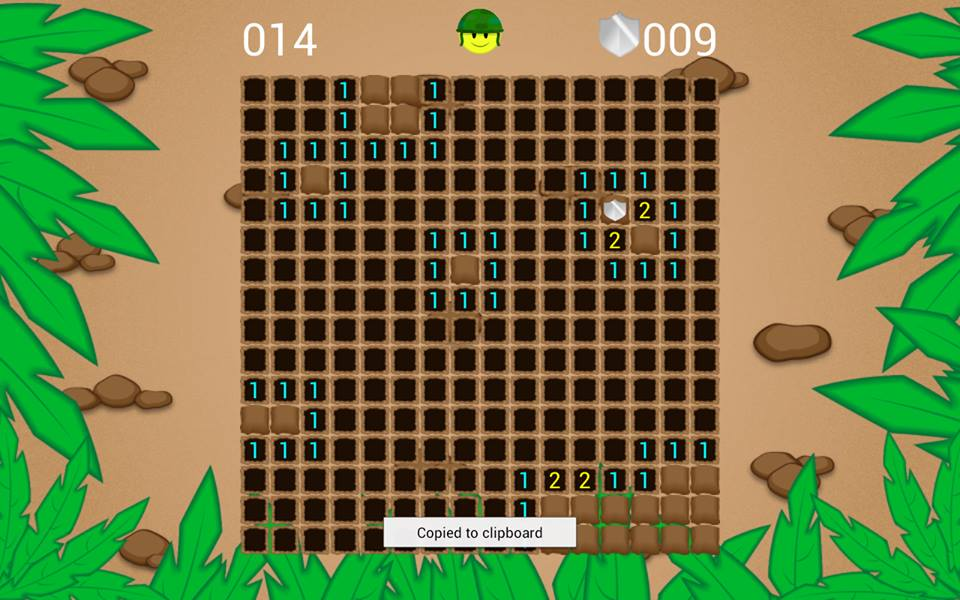
\includegraphics[width=1\textwidth]{images/screenshot7}
\end{center}
\end{minipage}
\end{figure}

\begin{figure}[h!]
\begin{minipage}{0.5 \textwidth}
Si presionamos una mina nos aparecerá un mensaje el cual nos indica que hemos perdido destapando asi todas las posiciones de las minas.
\end{minipage}
\hfill \begin{minipage}{6.5cm}
\begin{center}
 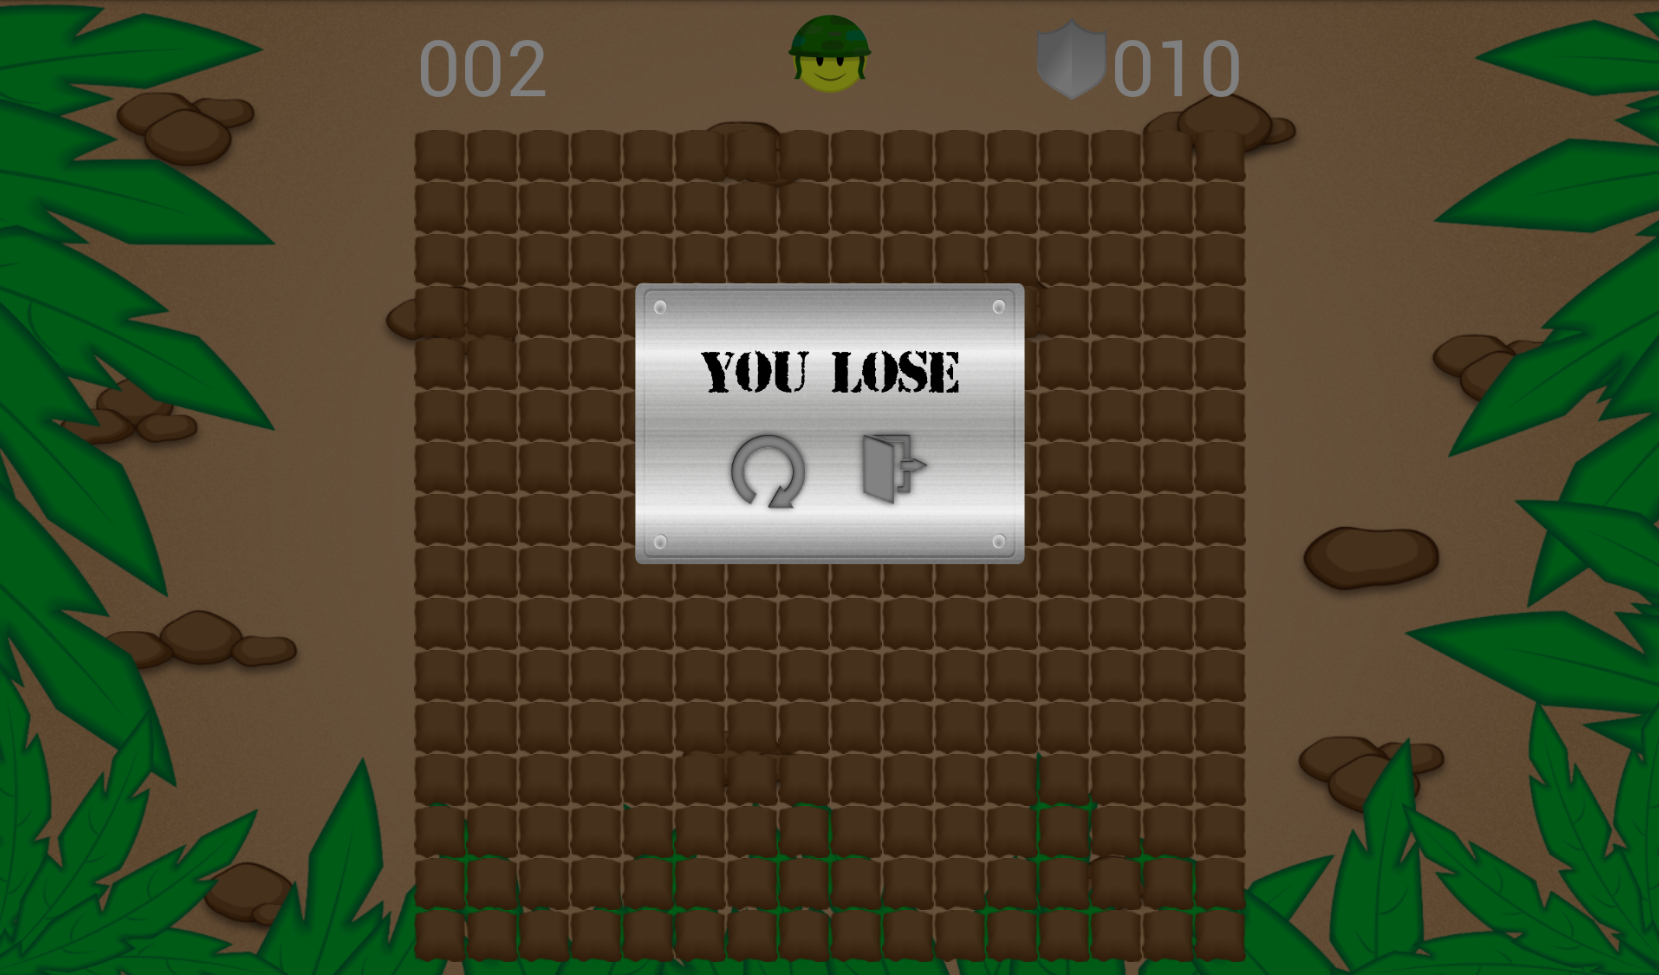
\includegraphics[width=1\textwidth]{images/screenshot8}
\end{center}
\end{minipage}
\end{figure}

\begin{figure}[h!]
\begin{minipage}{0.5 \textwidth}
En cambio si logramos encontrar la ubicación de todas las minas y taparlas con los escudos nos saldra un diálogo en el cual nos pedirá nuestro nombre para ser guardado entre los score del juego de acuerdo al nivel escojido y el puntaje logrado (para este caso el tiempo transcurrido).
\end{minipage}
\hfill \begin{minipage}{6.5cm}
\begin{center}
 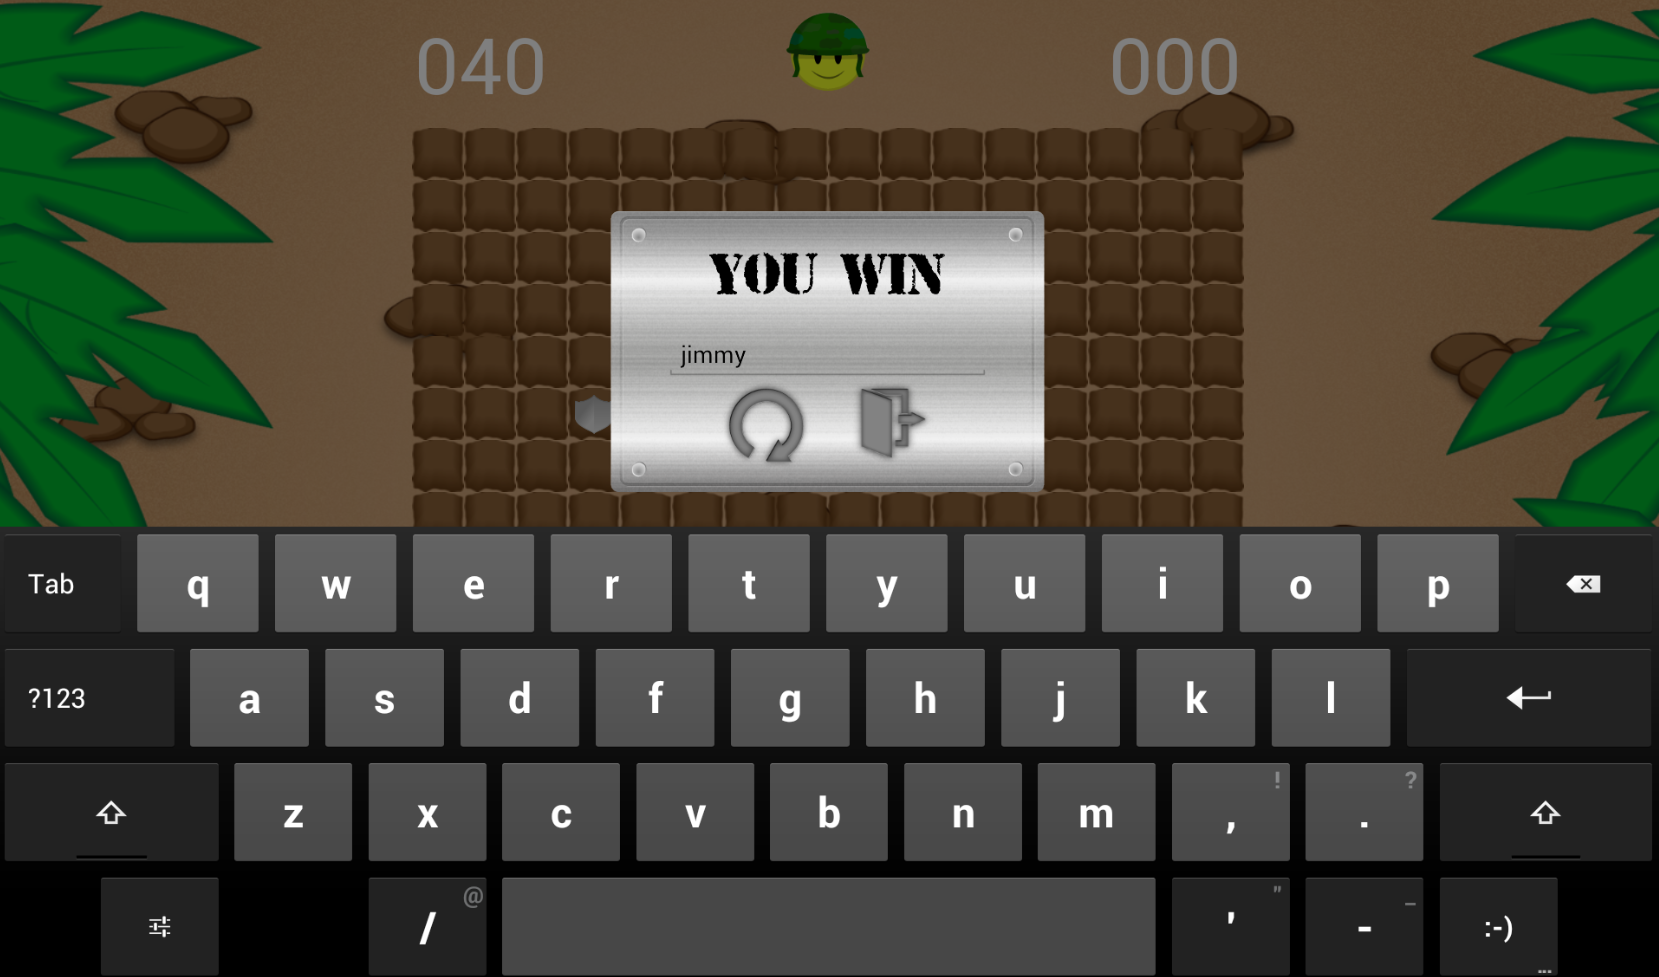
\includegraphics[width=1\textwidth]{images/screenshot9}
\end{center}
\end{minipage}
\end{figure}

\begin{figure}[h!]
\begin{minipage}{0.5 \textwidth}
En ambos casos sea gane o pierde se nos dara la opción como de reintentar el nivel  o regresar al menú según lo deseado. También tenemos nuestras 3 listas con los respectivos puntajes altos de cada nivel.
\end{minipage}
\hfill \begin{minipage}{6.5cm}
\begin{center}
 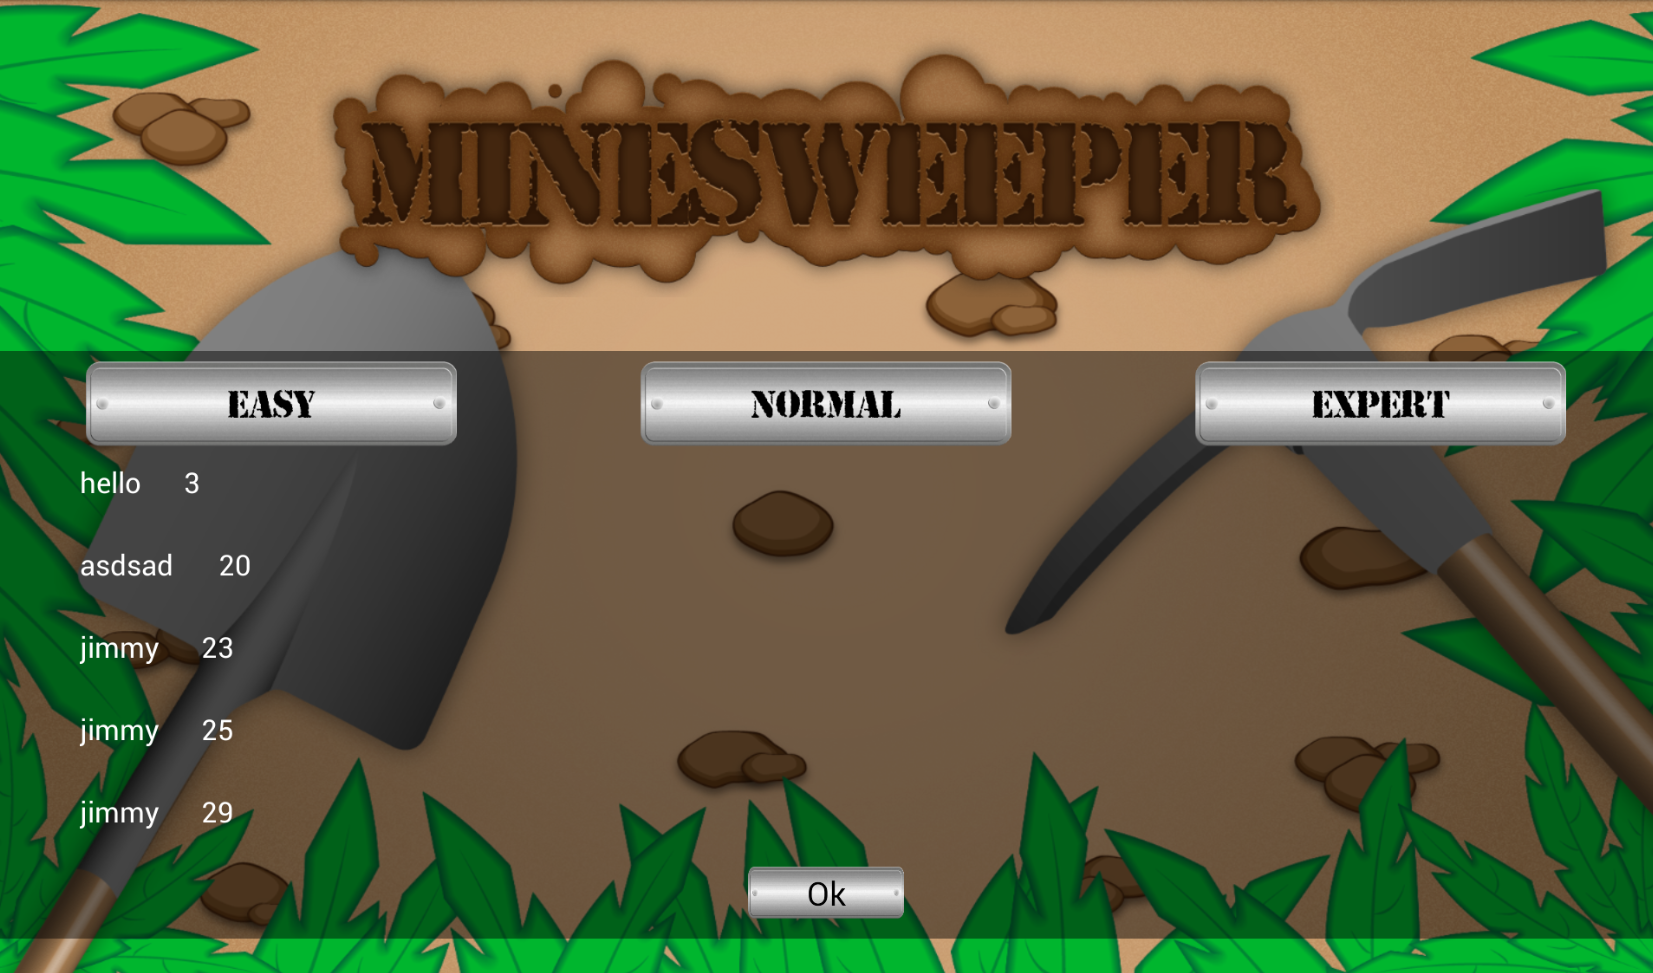
\includegraphics[width=1\textwidth]{images/screenshot10}
\end{center}
\end{minipage}
\end{figure}
\paragraph{}
\paragraph{}
\paragraph{} 
\paragraph{} 
\paragraph{} 
\paragraph{} 
\paragraph{}
\paragraph{}

\section{Conclusiones}
\begin{enumerate}
\item
En lo que respecta a diseño conocimos una nueva propiedad de ubicacion que posee android llamada weight la cual consiste en que designas un peso a cada componente que se encuentre en un mismo contenedor y de esta manera mediante pesos compara si uno ocupara el doble de espacio que otro o tan solo el mismo sin necesidad de darle una posicion especifica en el layout(dpi)\cite{android}.
\item
La implementación de lo que respecta al almacenamiento de scores fue planteada en un principio de dos maneras mediante el uso de xml y de la base de dato que ofrece el framework de android. Las dos implementaciones fueron exitosas pero nos decidimos por hacer uso de la base de datos ya que era más eficiente, usaba menos espacio, y más facil de implementar \cite{sql} \cite{xml}
\item
La implementación en android del zoom no pudo darse, talvez por falta de conocimiento acerca de que exactamente buscar, se trato escalando el ancho y alto de los botones pero esto afectaba drásticamente el diseño debido al {\textbf{layout}} en el que se encontraba.
\end{enumerate}

\bibliography{referencias}
\end{document}